
%%--------------------------------------------------
%% Serway: Physics for Scientists and Engineers
%%--------------------------------------------------


%% Chapter 09: Linear Momentum and Collisions
%%--------------------------------------------------


%% Table of Contents
%%--------------------------------------------------

%% 9.1 Linear Momentum and Its Conservation
%% 9.2 Impulse and Momentum
%% 9.3 Collisions in One Dimension
%% 9.4 Collisions in Two Dimensions
%% 9.5 The Center of Mass
%% 9.6 Motion of a System of Particles
%% 9.7 Deformable Systems
%% 9.8 Rocket Propulsion


%% Serway Multiple Choice Questions
%%--------------------------------------------------
\element{serway-mc}{
\begin{question}{serway-ch09-q01}
    A \SI{2000}{\kilo\gram} truck traveling at a speed of \SI{6.0}{\meter\per\second} makes a \ang{90} turn in a time of \SI{4.0}{\second} and emerges from this turn with a speed of \SI{4.0}{\meter\per\second}.
    What is the magnitude of the average resultant force on the truck during this turn?
    \begin{multicols}{3}
    \begin{choices}
        \wrongchoice{\SI{4.0}{\kilo\newton}}
        \wrongchoice{\SI{5.0}{\kilo\newton}}
      \correctchoice{\SI{3.6}{\kilo\newton}}
        \wrongchoice{\SI{6.4}{\kilo\newton}}
        \wrongchoice{\SI{0.67}{\kilo\newton}}
    \end{choices}
    \end{multicols}
\end{question}
}

\element{serway-mc}{
\begin{question}{serway-ch09-q02}
    A \SI{1.2}{\kilo\gram} object moving with a speed of \SI{8.0}{\meter\per\second} collides perpendicularly with a wall and emerges with a speed of \SI{6.0}{\meter\per\second} in the opposite direction.
    If the object is in contact with the wall for \SI{2.0}{\milli\second},
        what is the magnitude of the average force on the object by the wall?
    \begin{multicols}{3}
    \begin{choices}
        \wrongchoice{\SI{9.8}{\kilo\newton}}
      \correctchoice{\SI{8.4}{\kilo\newton}}
        \wrongchoice{\SI{7.7}{\kilo\newton}}
        \wrongchoice{\SI{9.1}{\kilo\newton}}
        \wrongchoice{\SI{1.2}{\kilo\newton}}
    \end{choices}
    \end{multicols}
\end{question}
}

\element{serway-mc}{
\begin{question}{serway-ch09-q03}
    A \SI{1.5}{\kilo\gram} playground ball is moving with a velocity of \SI{3.0}{\meter\per\second} directed \ang{30} below the horizontal just before it strikes a horizontal surface.
    The ball leaves this surface \SI{0.50}{\second} later with a velocity of \SI{2.0}{\meter\per\second} directed \ang{60} above the horizontal.
    What is the magnitude of the average resultant force on the ball?
    \begin{multicols}{3}
    \begin{choices}
        \wrongchoice{\SI{14}{\newton}}
      \correctchoice{\SI{11}{\newton}}
        \wrongchoice{\SI{18}{\newton}}
        \wrongchoice{\SI{22}{\newton}}
        \wrongchoice{\SI{3.0}{\newton}}
    \end{choices}
    \end{multicols}
\end{question}
}

\element{serway-mc}{
\begin{question}{serway-ch09-q04}
    The only force acting on a \SI{2.0}{\kilo\gram} object moving along the $x$ axis is shown.
    \begin{center}
    \begin{tikzpicture}
        \begin{axis}[
            axis y line=left,
            axis x line=middle,
            axis line style={->},
            xlabel={$t$},
            x unit=\si{\second},
            xtick={1,2,3,4},
            ylabel={$F_x$},
            y unit=\si{\newton},
            ytick={-8,-4,0,4},
            grid=major,
            xmin=0,xmax=5,
            ymin=-9,ymax=5,
            width=0.95\columnwidth,
            height=0.50\columnwidth,
        ]
        \addplot[line width=1pt,mark=\empty] coordinates { (0,4) (1,4) (4,-8) (5,-8) };
        \end{axis}
    \end{tikzpicture}
    \end{center}
    If the velocity $v_x$ is \SI{-2.0}{\meter\per\second} at $t=0$,
        what is the velocity at $t=\SI{4.0}{\second}$?
    \begin{multicols}{3}
    \begin{choices}
        \wrongchoice{\SI{-2.0}{\meter\per\second}}
        \wrongchoice{\SI{-4.0}{\meter\per\second}}
      \correctchoice{\SI{-3.0}{\meter\per\second}}
        \wrongchoice{\SI{+1.0}{\meter\per\second}}
        \wrongchoice{\SI{+5.0}{\meter\per\second}}
    \end{choices}
    \end{multicols}
\end{question}
}

\element{serway-mc}{
\begin{question}{serway-ch09-q05}
    The only force acting on a \SI{2.0}{\kilo\gram} object moving along the $x$ axis is shown.
    \begin{center}
    \begin{tikzpicture}
        \begin{axis}[
            axis y line=left,
            axis x line=middle,
            axis line style={->},
            xlabel={$t$},
            x unit=\si{\second},
            xtick={1,2,3,4},
            ylabel={$F_x$},
            y unit=\si{\newton},
            ytick={-8,0,8,16},
            grid=major,
            xmin=0,xmax=5,
            ymin=-9,ymax=17,
            width=0.95\columnwidth,
            height=0.50\columnwidth,
        ]
        \addplot[line width=1pt,mark=\empty] coordinates { (0,-8) (1,-8) (4,16) (5,16) };
        \end{axis}
    \end{tikzpicture}
    \end{center}
    If the velocity $v_x$ is \SI{+2.0}{\meter\per\second} at $t=0$,
        what is the velocity at $t=\SI{4.0}{\second}$?
    \begin{multicols}{3}
    \begin{choices}
      \correctchoice{\SI{+4.0}{\meter\per\second}}
        \wrongchoice{\SI{+5.0}{\meter\per\second}}
        \wrongchoice{\SI{+6.0}{\meter\per\second}}
        \wrongchoice{\SI{+7.0}{\meter\per\second}}
        \wrongchoice{\SI{+2.0}{\meter\per\second}}
    \end{choices}
    \end{multicols}
\end{question}
}

\element{serway-mc}{
\begin{question}{serway-ch09-q06}
    The speed of a \SI{2.0}{\kilo\gram} object changes from \SI{30}{\meter\per\second} to \SI{40}{\meter\per\second} during a \SI{5.0}{\second} time interval.
    During this same time interval,
        the velocity of the object changes its direction by \ang{90}.
    What is the magnitude of the average total force acting on the object during this time interval?
    \begin{multicols}{3}
    \begin{choices}
        \wrongchoice{\SI{30}{\newton}}
      \correctchoice{\SI{20}{\newton}}
        \wrongchoice{\SI{40}{\newton}}
        \wrongchoice{\SI{50}{\newton}}
        \wrongchoice{\SI{6.0}{\newton}}
    \end{choices}
    \end{multicols}
\end{question}
}

\element{serway-mc}{
\begin{question}{serway-ch09-q07}
    A \SI{3.0}{\kilo\gram} ball with an initial velocity of $(4\hat{\imath}+3\hat{\jmath})\,\si{\meter\per\second}$ collides with a wall and rebounds with a velocity of $(-4\hat{\imath}+3\hat{\jmath})\,\si{\meter\per\second}$.
    What is the impulse exerted on the ball by the wall?
    \begin{multicols}{2}
    \begin{choices}
        \wrongchoice{$+24\hat{\imath}\,\si{\newton\second}$}
      \correctchoice{$-24\hat{\imath}\,\si{\newton\second}$}
        \wrongchoice{$+18\hat{\jmath}\,\si{\newton\second}$}
        \wrongchoice{$-18\hat{\jmath}\,\si{\newton\second}$}
        \wrongchoice{$+8.0\hat{\imath}\,\si{\newton\second}$}
    \end{choices}
    \end{multicols}
\end{question}
}

\element{serway-mc}{
\begin{question}{serway-ch09-q08}
    A \SI{2.4}{\kilo\gram} ball falling vertically hits the floor with a speed of \SI{2.5}{\meter\per\second} and rebounds with a speed of \SI{1.5}{\meter\per\second}.
    What is the magnitude of the impulse exerted on the ball by the floor?
    \begin{multicols}{3}
    \begin{choices}
      \correctchoice{\SI{9.6}{\newton\second}}
        \wrongchoice{\SI{2.4}{\newton\second}}
        \wrongchoice{\SI{6.4}{\newton\second}}
        \wrongchoice{\SI{1.6}{\newton\second}}
        \wrongchoice{\SI{1.0}{\newton\second}}
    \end{choices}
    \end{multicols}
\end{question}
}

\element{serway-mc}{
\begin{question}{serway-ch09-q09}
    An \SI{8.0}{\kilo\gram} object moving \SI{4.0}{\meter\per\second} in the positive $x$ direction has a one-dimensional collision with a \SI{2.0}{\kilo\gram} object moving \SI{3.0}{\meter\per\second} in the opposite direction.
    The final velocity of the \SI{8.0}{\kilo\gram} object is \SI{2.0}{\meter\per\second} in the positive $x$ direction.
    What is the total kinetic energy of the two-mass system after the collision?
    \begin{multicols}{3}
    \begin{choices}
        \wrongchoice{\SI{32}{\joule}}
        \wrongchoice{\SI{52}{\joule}}
      \correctchoice{\SI{41}{\joule}}
        \wrongchoice{\SI{25}{\joule}}
        \wrongchoice{\SI{29}{\joule}}
    \end{choices}
    \end{multicols}
\end{question}
}

\element{serway-mc}{
\begin{question}{serway-ch09-q10}
    A \SI{1.6}{\kilo\gram} ball is attached to the end of a \SI{0.40}{\meter} string to form a pendulum.
    This pendulum is released from rest with the string horizontal.
    At the lowest point of its swing,
        when it is moving horizontally,
        the ball collides with a \SI{0.80}{\kilo\gram} block initially at rest on a horizontal frictionless surface.
    The speed of the block just after the collision is \SI{3.0}{\meter\per\second}.
    What is the speed of the ball just after the collision?
    \begin{multicols}{3}
    \begin{choices}
        \wrongchoice{\SI{1.7}{\meter\per\second}}
        \wrongchoice{\SI{1.1}{\meter\per\second}}
        \wrongchoice{\SI{1.5}{\meter\per\second}}
      \correctchoice{\SI{1.3}{\meter\per\second}}
        \wrongchoice{\SI{2.1}{\meter\per\second}}
    \end{choices}
    \end{multicols}
\end{question}
}

\element{serway-mc}{
\begin{question}{serway-ch09-q11}
    A \SI{4.0}{\kilo\gram} particle is moving horizontally with a speed of \SI{5.0}{\meter\per\second} when it strikes a vertical wall.
    The particle rebounds with a speed of \SI{3.0}{\meter\per\second}.
    What is the magnitude of the impulse delivered to the particle?
    \begin{multicols}{3}
    \begin{choices}
        \wrongchoice{\SI{24}{\newton\second}}
      \correctchoice{\SI{32}{\newton\second}}
        \wrongchoice{\SI{40}{\newton\second}}
        \wrongchoice{\SI{30}{\newton\second}}
        \wrongchoice{\SI{8.0}{\newton\second}}
    \end{choices}
    \end{multicols}
\end{question}
}

\element{serway-mc}{
\begin{question}{serway-ch09-q12}
    A \SI{2.0}{\kilo\gram} object moving with a velocity of \SI{5.0}{\meter\per\second} in the positive $x$ direction strikes and sticks to a \SI{3.0}{\kilo\gram} object moving with a speed of \SI{2.0}{\meter\per\second} in the same direction.
    How much kinetic energy is lost in this collision?
    \begin{multicols}{3}
    \begin{choices}
        \wrongchoice{\SI{2.4}{\joule}}
        \wrongchoice{\SI{9.6}{\joule}}
      \correctchoice{\SI{5.4}{\joule}}
        \wrongchoice{\SI{0.6}{\joule}}
        \wrongchoice{\SI{6.0}{\joule}}
    \end{choices}
    \end{multicols}
\end{question}
}

\element{serway-mc}{
\begin{question}{serway-ch09-q13}
    A \SI{10}{\gram} bullet moving \SI{1000}{\meter\per\second} strikes and passes through a \SI{2.0}{\kilo\gram} block initially at rest, as shown.
    The bullet emerges from the block with a speed of \SI{400}{\meter\per\second}.
    \begin{center}
    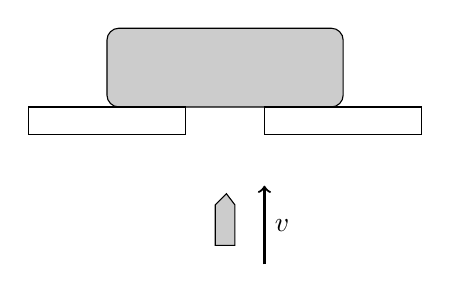
\begin{tikzpicture}
        %% Mass and platform
        \draw[fill=white!80!black,rounded corners=1ex] (-1.5,0) rectangle (1.5,1);
        \draw (-0.5,0) rectangle (-2.5,-1em);
        \draw (+0.5,0) rectangle (+2.5,-1em);
        %% Bullet
        \node[rectangle,rounded corners=1ex,minimum width=0.2cm,minimum height=0.5cm,anchor=center] (M) at (0,-1.5) {};
        \draw[fill=white!80!black] (M.north west) -- ++(45:0.2) -- (M.north east) -- (M.south east) -- (M.south west) -- cycle;
        \draw[thick,->] (+0.5,-2) -- ++(90:1) node[anchor=west,pos=0.5] {$v$};
    \end{tikzpicture}
    \end{center}
    To what maximum height will the block rise above its initial position?
    \begin{multicols}{3}
    \begin{choices}
        \wrongchoice{\SI{78}{\centi\meter}}
        \wrongchoice{\SI{66}{\centi\meter}}
        \wrongchoice{\SI{56}{\centi\meter}}
      \correctchoice{\SI{46}{\centi\meter}}
        \wrongchoice{\SI{37}{\centi\meter}}
    \end{choices}
    \end{multicols}
\end{question}
}

\element{serway-mc}{
\begin{question}{serway-ch09-q14}
    A \SI{12}{\gram} bullet moving horizontally strikes and remains in a \SI{3.0}{\kilo\gram} block initially at rest on the edge of a table.
    The block, which is initially \SI{80}{\centi\meter} above the floor,
        strikes the floor a horizontal distance of \SI{120}{\centi\meter} from its initial position.
    What was the initial speed of the bullet?
    \begin{multicols}{3}
    \begin{choices}
        \wrongchoice{\SI{0.68}{\kilo\meter\per\second}}
      \correctchoice{\SI{0.75}{\kilo\meter\per\second}}
        \wrongchoice{\SI{0.81}{\kilo\meter\per\second}}
        \wrongchoice{\SI{0.87}{\kilo\meter\per\second}}
        \wrongchoice{\SI{0.41}{\kilo\meter\per\second}}
    \end{choices}
    \end{multicols}
\end{question}
}

\element{serway-mc}{
\begin{question}{serway-ch09-q15}
    A \SI{6.0}{\kilo\gram} object moving \SI{5.0}{\meter\per\second} collides with and sticks to a \SI{2.0}{\kilo\gram} object.
    After the collision the composite object is moving \SI{2.0}{\meter\per\second} in a direction opposite to the initial direction of motion of the \SI{6.0}{\kilo\gram} object.
    Determine the speed of the \SI{2.0}{\kilo\gram} object before the collision.
    \begin{multicols}{3}
    \begin{choices}
        \wrongchoice{\SI{15}{\meter\per\second}}
        \wrongchoice{\SI{7.0}{\meter\per\second}}
        \wrongchoice{\SI{8.0}{\meter\per\second}}
      \correctchoice{\SI{23}{\meter\per\second}}
        \wrongchoice{\SI{11}{\meter\per\second}}
    \end{choices}
    \end{multicols}
\end{question}
}

\element{serway-mc}{
\begin{question}{serway-ch09-q16}
    A \SI{2.0}{\kilo\gram} object moving \SI{5.0}{\meter\per\second} collides with and sticks to an \SI{8.0}{\kilo\gram} object initially at rest.
    Determine the kinetic energy lost by the system as a result of this collision.
    \begin{multicols}{3}
    \begin{choices}
      \correctchoice{\SI{20}{\joule}}
        \wrongchoice{\SI{15}{\joule}}
        \wrongchoice{\SI{30}{\joule}}
        \wrongchoice{\SI{25}{\joule}}
        \wrongchoice{\SI{5.0}{\joule}}
    \end{choices}
    \end{multicols}
\end{question}
}

\element{serway-mc}{
\begin{question}{serway-ch09-q17}
    A \SI{1.6}{\kilo\gram} block is attached to the end of a \SI{2.0}{\meter} string to form a pendulum.
    The pendulum is released from rest when the string is horizontal.
    At the lowest point of its swing when it is moving horizontally,
        the block is hit by a \SI{10}{\gram} bullet moving horizontally in the opposite direction.
    The bullet remains in the block and causes the block to come to rest at the low point of its swing.
    What was the magnitude of the bullet's velocity just before hitting the block?
    \begin{multicols}{3}
    \begin{choices}
      \correctchoice{\SI{1.0}{\kilo\meter\per\second}}
        \wrongchoice{\SI{1.6}{\kilo\meter\per\second}}
        \wrongchoice{\SI{1.2}{\kilo\meter\per\second}}
        \wrongchoice{\SI{1.4}{\kilo\meter\per\second}}
        \wrongchoice{\SI{1.8}{\kilo\meter\per\second}}
    \end{choices}
    \end{multicols}
\end{question}
}

\element{serway-mc}{
\begin{question}{serway-ch09-q18}
    A \SI{3.0}{\kilo\gram} mass sliding on a frictionless surface has a velocity of \SI{5.0}{\meter\per\second} east when it undergoes a one-dimensional inelastic collision with a \SI{2.0}{\kilo\gram} mass that has an initial velocity of \SI{2.0}{\meter\per\second} west.
    After the collision the \SI{3.0}{\kilo\gram} mass has a velocity of \SI{1.0}{\meter\per\second} east.
    How much kinetic energy does the two-mass system lose during the collision?
    \begin{multicols}{3}
    \begin{choices}
        \wrongchoice{\SI{22}{\joule}}
      \correctchoice{\SI{24}{\joule}}
        \wrongchoice{\SI{26}{\joule}}
        \wrongchoice{\SI{20}{\joule}}
        \wrongchoice{\SI{28}{\joule}}
    \end{choices}
    \end{multicols}
\end{question}
}

\element{serway-mc}{
\begin{question}{serway-ch09-q19}
    A \SI{3.0}{\kilo\gram} mass is released from rest at point $A$ of a circular frictionless track of radius \SI{0.40}{\meter} as shown in the figure.
    The mass slides down the track and collides with a \SI{1.4}{\kilo\gram} mass that is initially at rest on a horizontal frictionless surface.
    \begin{center}
    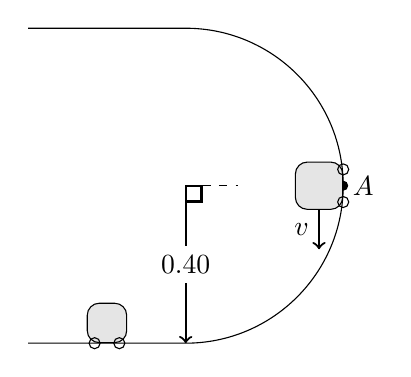
\begin{tikzpicture}
        %% Surface
        \draw (-2,2) -- (0,2) arc (90:-90:2) -- (-2,-2);
        %% Labels
        \draw[dashed] (0,0) -- ++(0:0.66);
        \draw[thick,->] (0,0) -- ++(270:2) node[anchor=center,fill=white,pos=0.5] {\SI{0.40}{\meter}};
        \draw[thick] (0,0) -- (0,-0.2) -- (0.2,-0.2) -- (0.2,0) -- cycle;
        \draw[fill] (0:2) circle (1.6pt) node[anchor=west] {$A$};
        %% Cart
        \node[draw,fill=white!90!black,rectangle,rounded corners=1ex,minimum size=0.6cm,anchor=south,rotate=90] (A) at (2,0) {};
        \node[draw,fill=white!90!black,rectangle,rounded corners=1ex,minimum size=0.5cm,anchor=south] (B) at (-1,-2) {};
        %% Wheels
        \draw (A.south west) ++(90:0.1) circle (2pt);
        \draw (A.south east) ++(270:0.1) circle (2pt);
        \draw (B.south west) ++(0:0.1) circle (2pt);
        \draw (B.south east) ++(180:0.1) circle (2pt);
        %\draw[thick,->] (A.north) ++(135:0.7) -- ++(270:1) node[anchor=west,pos=0.5] {$v$};
        \draw[thick,->] (A.west) -- ++(270:0.5) node[anchor=east,pos=0.5] {$v$};
    \end{tikzpicture}
    \end{center}
    If the masses stick together, what is their speed after the collision?
    \begin{multicols}{3}
    \begin{choices}
        \wrongchoice{\SI{2.1}{\meter\per\second}}
        \wrongchoice{\SI{1.7}{\meter\per\second}}
      \correctchoice{\SI{1.9}{\meter\per\second}}
        \wrongchoice{\SI{1.5}{\meter\per\second}}
        \wrongchoice{\SI{2.3}{\meter\per\second}}
    \end{choices}
    \end{multicols}
\end{question}
}

\element{serway-mc}{
\begin{question}{serway-ch09-q20}
    A \SI{3.0}{\kilo\gram} mass is sliding on a horizontal frictionless surface with a speed of \SI{3.0}{\meter\per\second} when it collides with a \SI{1.0}{\kilo\gram} mass initially at rest as shown in the figure.
    The masses stick together and slide up a frictionless circular track of radius \SI{0.40}{\meter}.
    \begin{center}
    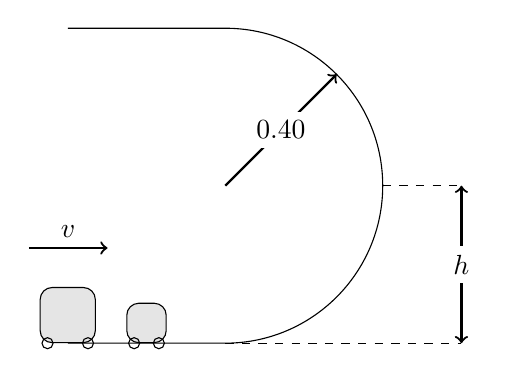
\begin{tikzpicture}
        %% Surface
        \draw (-2,2) -- (0,2) arc (90:-90:2) -- (-2,-2);
        %% Labels
        \draw[dashed] (2,0) -- ++(0:1);
        \draw[dashed] (0,-2) -- ++(0:3);
        \draw[thick,<->] (3,-2) -- ++(90:2) node[pos=0.5,anchor=center,fill=white] {$h$};
        \draw[thick,->] (0,0) -- ++(45:2) node[anchor=center,fill=white,pos=0.5] {\SI{0.40}{\meter}};
        %% Cart
        \node[draw,fill=white!90!black,rectangle,rounded corners=1ex,minimum size=0.7cm,anchor=south] (A) at (-2,-2) {};
        \node[draw,fill=white!90!black,rectangle,rounded corners=1ex,minimum size=0.5cm,anchor=south] (B) at (-1,-2) {};
        %% Wheels
        \draw (A.south west) ++(0:0.1) circle (2pt);
        \draw (A.south east) ++(180:0.1) circle (2pt);
        \draw (B.south west) ++(0:0.1) circle (2pt);
        \draw (B.south east) ++(180:0.1) circle (2pt);
        \draw[thick,->] (A.north) ++(135:0.7) -- ++(0:1) node[anchor=south,pos=0.5] {$v$};
    \end{tikzpicture}
    \end{center}
    To what maximum height, $h$, above the horizontal surface will the masses slide?
    \begin{multicols}{3}
    \begin{choices}
        \wrongchoice{\SI{0.18}{\meter}}
        \wrongchoice{\SI{0.15}{\meter}}
        \wrongchoice{\SI{0.21}{\meter}}
      \correctchoice{\SI{0.26}{\meter}}
        \wrongchoice{\SI{0.40}{\meter}}
    \end{choices}
    \end{multicols}
\end{question}
}

\element{serway-mc}{
\begin{question}{serway-ch09-q21}
    A \SI{10}{\gram} bullet moving horizontally with a speed of \SI{2.0}{\kilo\meter\per\second} strikes and passes through a \SI{4.0}{\kilo\gram} block moving with a speed of \SI{4.2}{\meter\per\second} in the opposite direction on a horizontal frictionless surface.
    If the block is brought to rest by the collision,
        what is the kinetic energy of the bullet as it emerges from the block?
    \begin{multicols}{3}
    \begin{choices}
      \correctchoice{\SI{0.51}{\kilo\joule}}
        \wrongchoice{\SI{0.29}{\kilo\joule}}
        \wrongchoice{\SI{0.80}{\kilo\joule}}
        \wrongchoice{\SI{0.13}{\kilo\joule}}
        \wrongchoice{\SI{20}{\kilo\joule}}
    \end{choices}
    \end{multicols}
\end{question}
}

\element{serway-mc}{
\begin{question}{serway-ch09-q22}
    A \SI{10}{\gram} bullet moving horizontally with a speed of \SI{1.8}{\kilo\meter\per\second} strikes and passes through a \SI{5.0}{\kilo\gram} block initially at rest on a horizontal frictionless surface.
    The bullet emerges from the block with a speed of \SI{1.0}{\kilo\meter\per\second}.
    What is the kinetic energy of the block immediately after the bullet emerges?
    \begin{multicols}{3}
    \begin{choices}
        \wrongchoice{\SI{8.0}{\joule}}
      \correctchoice{\SI{6.4}{\joule}}
        \wrongchoice{\SI{5.3}{\joule}}
        \wrongchoice{\SI{9.4}{\joule}}
        \wrongchoice{\SI{10}{\joule}}
    \end{choices}
    \end{multicols}
\end{question}
}

\element{serway-mc}{
\begin{question}{serway-ch09-q23}
    A pendulum consists of a \SI{2.0}{\kilo\gram} block hanging on a \SI{1.5}{\meter} length string.
    A \SI{10}{\gram} bullet moving with a horizontal velocity of \SI{900}{\meter\per\second} strikes,
        passes through, and emerges from the block (initially at rest) with a horizontal velocity of \SI{300}{\meter\per\second}.
    To what maximum height above its initial position will the block swing?
    \begin{multicols}{3}
    \begin{choices}
        \wrongchoice{\SI{32}{\centi\meter}}
        \wrongchoice{\SI{38}{\centi\meter}}
      \correctchoice{\SI{46}{\centi\meter}}
        \wrongchoice{\SI{27}{\centi\meter}}
        \wrongchoice{\SI{9}{\centi\meter}}
    \end{choices}
    \end{multicols}
\end{question}
}

\element{serway-mc}{
\begin{question}{serway-ch09-q24}
    A \SI{1.0}{\kilo\gram} ball is attached to the end of a \SI{2.5}{\meter} string to form a pendulum.
    This pendulum is released from rest with the string horizontal.
    At the lowest point in its swing when it is moving horizontally,
        the ball collides elastically with a \SI{2.0}{\kilo\gram} block initially at rest on a horizontal frictionless surface.
    What is the speed of the block just after the collision?
    \begin{multicols}{3}
    \begin{choices}
        \wrongchoice{\SI{2.3}{\meter\per\second}}
      \correctchoice{\SI{4.7}{\meter\per\second}}
        \wrongchoice{\SI{3.5}{\meter\per\second}}
        \wrongchoice{\SI{3.0}{\meter\per\second}}
        \wrongchoice{\SI{7.0}{\meter\per\second}}
    \end{choices}
    \end{multicols}
\end{question}
}

\element{serway-mc}{
\begin{question}{serway-ch09-q25}
    A \SI{3.0}{\kilo\gram} object moving in the positive $x$ direction has a one-dimensional elastic collision with a \SI{5.0}{\kilo\gram} object initially at rest.
    After the collision the \SI{5.0}{\kilo\gram} object has a velocity of \SI{6.0}{\meter\per\second} in the positive $x$ direction.
    What was the initial speed of the \SI{3.0}{\kilo\gram} object?
    \begin{multicols}{3}
    \begin{choices}
        \wrongchoice{\SI{6.0}{\meter\per\second}}
        \wrongchoice{\SI{7.0}{\meter\per\second}}
        \wrongchoice{\SI{4.5}{\meter\per\second}}
      \correctchoice{\SI{8.0}{\meter\per\second}}
        \wrongchoice{\SI{5.5}{\meter\per\second}}
    \end{choices}
    \end{multicols}
\end{question}
}

\element{serway-mc}{
\begin{question}{serway-ch09-q26}
    A \SI{3.0}{\kilo\gram} object moving \SI{8.0}{\meter\per\second} in the positive $x$ direction has a one-dimensional elastic collision with an object (mass = $M$) initially at rest.
    After the collision the object of unknown mass has a velocity of \SI{6.0}{\meter\per\second} in the positive $x$ direction.
    What is $M$?
    \begin{multicols}{3}
    \begin{choices}
        \wrongchoice{\SI{7.5}{\kilo\gram}}
      \correctchoice{\SI{5.0}{\kilo\gram}}
        \wrongchoice{\SI{6.0}{\kilo\gram}}
        \wrongchoice{\SI{4.2}{\kilo\gram}}
        \wrongchoice{\SI{8.0}{\kilo\gram}}
    \end{choices}
    \end{multicols}
\end{question}
}

\element{serway-mc}{
\begin{question}{serway-ch09-q27}
    A \SI{6.0}{\kilo\gram} object moving \SI{2.0}{\meter\per\second} in the positive $x$ direction has a one-dimensional elastic collision with a \SI{4.0}{\kilo\gram} object moving \SI{3.0}{\meter\per\second} in the opposite direction.
    What is the total kinetic energy of the two-mass system after the collision?
    \begin{multicols}{3}
    \begin{choices}
      \correctchoice{\SI{30}{\joule}}
        \wrongchoice{\SI{62}{\joule}}
        \wrongchoice{\SI{20}{\joule}}
        \wrongchoice{\SI{44}{\joule}}
        \wrongchoice{\SI{24}{\joule}}
    \end{choices}
    \end{multicols}
\end{question}
}

\element{serway-mc}{
\begin{question}{serway-ch09-q28}
    Two blocks with masses \SI{2.0}{\kilo\gram} and \SI{3.0}{\kilo\gram} are placed on a horizontal frictionless surface.
    A light spring is placed in a horizontal position between the blocks.
    The blocks are pushed together, compressing the spring, and then released from rest.
    After contact with the spring ends, the \SI{3.0}{\kilo\gram} mass has a speed of \SI{2.0}{\meter\per\second}.
    How much potential energy was stored in the spring when the blocks were released?
    \begin{multicols}{3}
    \begin{choices}
      \correctchoice{\SI{15}{\joule}}
        \wrongchoice{\SI{3.0}{\joule}}
        \wrongchoice{\SI{6.0}{\joule}}
        \wrongchoice{\SI{12}{\joule}}
        \wrongchoice{\SI{9.0}{\joule}}
    \end{choices}
    \end{multicols}
\end{question}
}

\element{serway-mc}{
\begin{question}{serway-ch09-q29}
    An \SI{80}{\gram} particle moving with an initial speed of \SI{50}{\meter\per\second} in the positive $x$ direction strikes and sticks to a \SI{60}{\gram} particle moving \SI{50}{\meter\per\second} in the positive $y$ direction.
    How much kinetic energy is lost in this collision?
    \begin{multicols}{3}
    \begin{choices}
        \wrongchoice{\SI{96}{\joule}}
        \wrongchoice{\SI{89}{\joule}}
        \wrongchoice{\SI{175}{\joule}}
      \correctchoice{\SI{86}{\joule}}
        \wrongchoice{\SI{110}{\joule}}
    \end{choices}
    \end{multicols}
\end{question}
}

\element{serway-mc}{
\begin{question}{serway-ch09-q30}
    A \SI{2.0}{\kilo\gram} object moving \SI{3.0}{\meter\per\second} strikes a \SI{1.0}{\kilo\gram} object initially at rest.
    Immediately after the collision,
        the \SI{2.0}{\kilo\gram} object has a velocity of \SI{1.5}{\meter\per\second} directed \ang{30} from its initial direction of motion.
    What is the $x$-component of the velocity of the \SI{1.0}{\kilo\gram} object just after the collision?
    \begin{multicols}{3}
    \begin{choices}
        \wrongchoice{\SI{3.7}{\meter\per\second}}
      \correctchoice{\SI{3.4}{\meter\per\second}}
        \wrongchoice{\SI{1.5}{\meter\per\second}}
        \wrongchoice{\SI{2.4}{\meter\per\second}}
        \wrongchoice{\SI{4.1}{\meter\per\second}}
    \end{choices}
    \end{multicols}
\end{question}
}

\element{serway-mc}{
\begin{question}{serway-ch09-q31}
    A \SI{2.0}{\kilo\gram} object moving \SI{3.0}{\meter\per\second} strikes a \SI{1.0}{\kilo\gram} object initially at rest.
    Immediately after the collision,
        the \SI{2.0}{\kilo\gram} object has a velocity of \SI{1.5}{\meter\per\second} directed \ang{30} from its initial direction of motion.
    What is the $y$-component of the velocity of the \SI{1.0}{\kilo\gram} object just after the collision?
    \begin{multicols}{3}
    \begin{choices}
        \wrongchoice{\SI{-3.7}{\meter\per\second}}
        \wrongchoice{\SI{-3.4}{\meter\per\second}}
      \correctchoice{\SI{-1.5}{\meter\per\second}}
        \wrongchoice{\SI{-2.4}{\meter\per\second}}
        \wrongchoice{\SI{-4.1}{\meter\per\second}}
    \end{choices}
    \end{multicols}
\end{question}
}

\element{serway-mc}{
\begin{question}{serway-ch09-q32}
    A \SI{6.0}{\kilo\gram} object, initially at rest in free space,
        ``explodes'' into three segments of equal mass.
    Two of these segments are observed to be moving with equal speeds of \SI{20}{\meter\per\second} with an angle of \ang{60} between their directions of motion.
    How much kinetic energy is released in this explosion?
    \begin{multicols}{3}
    \begin{choices}
        \wrongchoice{\SI{2.4}{\kilo\joule}}
        \wrongchoice{\SI{2.9}{\kilo\joule}}
      \correctchoice{\SI{2.0}{\kilo\joule}}
        \wrongchoice{\SI{3.4}{\kilo\joule}}
        \wrongchoice{\SI{1.2}{\kilo\joule}}
    \end{choices}
    \end{multicols}
\end{question}
}

\element{serway-mc}{
\begin{question}{serway-ch09-q33}
    A \SI{5.0}{\gram} particle moving \SI{60}{\meter\per\second} collides with a \SI{2.0}{\gram} particle initially at rest.
    After the collision each of the particles has a velocity that is directed \ang{30} from the original direction of motion of the \SI{5.0}{\gram} particle.
    What is the speed of the \SI{2.0}{\gram} particle after the collision?
    \begin{multicols}{3}
    \begin{choices}
        \wrongchoice{\SI{72}{\meter\per\second}}
      \correctchoice{\SI{87}{\meter\per\second}}
        \wrongchoice{\SI{79}{\meter\per\second}}
        \wrongchoice{\SI{94}{\meter\per\second}}
        \wrongchoice{\SI{67}{\meter\per\second}}
    \end{choices}
    \end{multicols}
\end{question}
}

\element{serway-mc}{
\begin{question}{serway-ch09-q34}
    A \SI{1.0}{\kilo\gram} object moving \SI{9.0}{\meter\per\second} collides with a \SI{2.0}{\kilo\gram} object moving \SI{6.0}{\meter\per\second} in a direction that is perpendicular to the initial direction of motion of the \SI{1.0}{\kilo\gram} object.
    The two masses remain together after the collision,
        and this composite object then collides with and sticks to a \SI{3.0}{\kilo\gram} object.
    After these collisions, the final composite (\SI{6.0}{\kilo\gram}) object remains at rest.
    What was the speed of the \SI{3.0}{\kilo\gram} object before the collisions?
    \begin{multicols}{3}
    \begin{choices}
        \wrongchoice{\SI{15}{\meter\per\second}}
        \wrongchoice{\SI{10}{\meter\per\second}}
      \correctchoice{\SI{5.0}{\meter\per\second}}
        \wrongchoice{\SI{20}{\meter\per\second}}
        \wrongchoice{\SI{25}{\meter\per\second}}
    \end{choices}
    \end{multicols}
\end{question}
}

\element{serway-mc}{
\begin{question}{serway-ch09-q35}
    A \SI{3.0}{\kilo\gram} mass sliding on a frictionless surface explodes into three \SI{1.0}{\kilo\gram} masses.
    After the explosion the velocities of the three masses are:
        (1) \SI{9.0}{\meter\per\second}, north; (2) \SI{4.0}{\meter\per\second}, \ang{30} south of west; and (3) \SI{4.0}{\meter\per\second}, \ang{30} south of east.
    What was the magnitude of the original velocity of the \SI{3.0}{\kilo\gram} mass?
    \begin{multicols}{3}
    \begin{choices}
      \correctchoice{\SI{1.7}{\meter\per\second}}
        \wrongchoice{\SI{1.0}{\meter\per\second}}
        \wrongchoice{\SI{1.3}{\meter\per\second}}
        \wrongchoice{\SI{2.0}{\meter\per\second}}
        \wrongchoice{\SI{2.8}{\meter\per\second}}
    \end{choices}
    \end{multicols}
\end{question}
}

\element{serway-mc}{
\begin{question}{serway-ch09-q36}
    A \SI{3.0}{\kilo\gram} mass moving in the positive x direction with a speed of \SI{10}{\meter\per\second} collides with a \SI{6.0}{\kilo\gram} mass initially at rest.
    After the collision, the speed of the \SI{3.0}{\kilo\gram} mass is \SI{8.0}{\meter\per\second},
        and its velocity vector makes an angle of \ang{35} with the positive $x$ axis.
    What is the magnitude of the velocity of the \SI{6.0}{\kilo\gram} mass after the collision?
    \begin{multicols}{3}
    \begin{choices}
        \wrongchoice{\SI{2.2}{\meter\per\second}}
      \correctchoice{\SI{2.9}{\meter\per\second}}
        \wrongchoice{\SI{4.2}{\meter\per\second}}
        \wrongchoice{\SI{3.5}{\meter\per\second}}
        \wrongchoice{\SI{4.7}{\meter\per\second}}
    \end{choices}
    \end{multicols}
\end{question}
}

\element{serway-mc}{
\begin{question}{serway-ch09-q37}
    A \SI{5.0}{\kilo\gram} mass with an initial velocity of \SI{4.0}{\meter\per\second}, east collides with a \SI{4.0}{\kilo\gram} mass with an initial velocity of \SI{3.0}{\meter\per\second}, west.
    After the collision the \SI{5.0}{\kilo\gram} mass has a velocity of \SI{1.2}{\meter\per\second}, south.
    What is the magnitude of the velocity of the \SI{4.0}{\kilo\gram} mass after the collision?
    \begin{multicols}{3}
    \begin{choices}
        \wrongchoice{\SI{2.0}{\meter\per\second}}
        \wrongchoice{\SI{1.5}{\meter\per\second}}
        \wrongchoice{\SI{1.0}{\meter\per\second}}
      \correctchoice{\SI{2.5}{\meter\per\second}}
        \wrongchoice{\SI{3.0}{\meter\per\second}}
    \end{choices}
    \end{multicols}
\end{question}
}

\element{serway-mc}{
\begin{question}{serway-ch09-q38}
    A \SI{4.0}{\kilo\gram} mass has a velocity of \SI{4.0}{\meter\per\second},
        east when it explodes into two \SI{2.0}{\kilo\gram} masses.
    After the explosion one of the masses has a velocity of \SI{3.0}{\meter\per\second} at an angle of \ang{60} north of east.
    What is the magnitude of the velocity of the other mass after the explosion?
    \begin{multicols}{3}
    \begin{choices}
        \wrongchoice{\SI{7.9}{\meter\per\second}}
        \wrongchoice{\SI{8.9}{\meter\per\second}}
      \correctchoice{\SI{7.0}{\meter\per\second}}
        \wrongchoice{\SI{6.1}{\meter\per\second}}
        \wrongchoice{\SI{6.7}{\meter\per\second}}
    \end{choices}
    \end{multicols}
\end{question}
}

\element{serway-mc}{
\begin{question}{serway-ch09-q39}
    A \SI{4.2}{\kilo\gram} object, initially at rest, ``explodes'' into three objects of equal mass.
    Two of these are determined to have velocities of equal magnitudes (\SI{5.0}{\meter\per\second}) with directions that differ by \ang{90}.
    How much kinetic energy was released in the explosion?
    \begin{multicols}{3}
    \begin{choices}
      \correctchoice{\SI{70}{\joule}}
        \wrongchoice{\SI{53}{\joule}}
        \wrongchoice{\SI{60}{\joule}}
        \wrongchoice{\SI{64}{\joule}}
        \wrongchoice{\SI{35}{\joule}}
    \end{choices}
    \end{multicols}
\end{question}
}

\element{serway-mc}{
\begin{question}{serway-ch09-q40}
    A \SI{4.0}{\kilo\gram} mass, initially at rest on a horizontal frictionless surface, is struck by a \SI{2.0}{\kilo\gram} mass moving along the $x$ axis with a speed of \SI{8.0}{\meter\per\second}.
    After the collision, the \SI{2.0}{\kilo\gram} mass has a speed of \SI{4.0}{\meter\per\second} at an angle of \ang{37} from the positive $x$ axis.
    What is the speed of the \SI{4.0}{\kilo\gram} mass after the collision?
    \begin{multicols}{3}
    \begin{choices}
        \wrongchoice{\SI{2.0}{\meter\per\second}}
      \correctchoice{\SI{2.7}{\meter\per\second}}
        \wrongchoice{\SI{4.9}{\meter\per\second}}
        \wrongchoice{\SI{2.4}{\meter\per\second}}
        \wrongchoice{\SI{3.6}{\meter\per\second}}
    \end{choices}
    \end{multicols}
\end{question}
}

\element{serway-mc}{
\begin{question}{serway-ch09-q41}
    At an instant when a particle of mass \SI{50}{\gram} has an acceleration of \SI{80}{\meter\per\second\squared} in the positive $x$ direction,
        a \SI{75}{\gram} particle has an acceleration of \SI{40}{\meter\per\second\squared} in the positive $y$ direction.
    What is the magnitude of the acceleration of the center of mass of this two-particle system at this instant?
    \begin{multicols}{3}
    \begin{choices}
        \wrongchoice{\SI{60}{\meter\per\second\squared}}
        \wrongchoice{\SI{56}{\meter\per\second\squared}}
      \correctchoice{\SI{40}{\meter\per\second\squared}}
        \wrongchoice{\SI{50}{\meter\per\second\squared}}
        \wrongchoice{\SI{46}{\meter\per\second\squared}}
    \end{choices}
    \end{multicols}
\end{question}
}

\element{serway-mc}{
\begin{question}{serway-ch09-q42}
    At an instant when a particle of mass \SI{80}{\gram} has a velocity of \SI{25}{\meter\per\second} in the positive $y$ direction, a \SI{75}{\gram} particle has a velocity of \SI{20}{\meter\per\second} in the positive x direction.
    What is the speed of the center of mass of this two-particle system at this instant?
    \begin{multicols}{3}
    \begin{choices}
      \correctchoice{\SI{16}{\meter\per\second}}
        \wrongchoice{\SI{45}{\meter\per\second}}
        \wrongchoice{\SI{23}{\meter\per\second}}
        \wrongchoice{\SI{20}{\meter\per\second}}
        \wrongchoice{\SI{36}{\meter\per\second}}
    \end{choices}
    \end{multicols}
\end{question}
}

\element{serway-mc}{
\begin{question}{serway-ch09-q43}
    Three particles are placed in the $xy$ plane.
    A \SI{40}{\gram} particle is located at $\left(3,4\right)\,\si{\meter}$,
        and a \SI{50}{\gram} particle is positioned at $\left(-2,-6\right)\,\si{\meter}$.
    Where must a \SI{20}{\gram} particle be placed so that the center of mass of this three-particle system is located at the origin?
    \begin{multicols}{2}
    \begin{choices}
        \wrongchoice{$\left(-1,-3\right)\,\si{\meter}$}
        \wrongchoice{$\left(-1,+2\right)\,\si{\meter}$}
        \wrongchoice{$\left(-1,+12\right)\,\si{\meter}$}
      \correctchoice{$\left(-1,+7\right)\,\si{\meter}$}
        \wrongchoice{$\left(-1,+3\right)\,\si{\meter}$}
    \end{choices}
    \end{multicols}
\end{question}
}

\element{serway-mc}{
\begin{question}{serway-ch09-q44}
    A rocket engine consumes \SI{450}{\kilo\gram} of fuel per minute.
    If the exhaust speed of the ejected fuel is \SI{5.2}{\kilo\meter\per\second},
        what is the thrust of the rocket?
    \begin{multicols}{3}
    \begin{choices}
        \wrongchoice{\SI{42}{\kilo\newton}}
      \correctchoice{\SI{39}{\kilo\newton}}
        \wrongchoice{\SI{45}{\kilo\newton}}
        \wrongchoice{\SI{48}{\kilo\newton}}
        \wrongchoice{\SI{35}{\kilo\newton}}
    \end{choices}
    \end{multicols}
\end{question}
}

\element{serway-mc}{
\begin{question}{serway-ch09-q45}
    A rocket with an initial mass of \SI{1000}{\kilo\gram} adjusts its thrust by varying the rate at which mass is ejected.
    The ejection speed relative to the rocket is \SI{40}{\kilo\meter\per\second}.
    If the acceleration of the rocket is to have a magnitude of \SI{20}{\meter\per\second\squared} at an instant when its mass is \SI{80}{\percent} of the original mass,
        at what rate is mass being ejected at that instant?
    Ignore any external forces on the rocket.
    \begin{multicols}{3}
    \begin{choices}
      \correctchoice{\SI{0.40}{\kilo\gram\per\second}}
        \wrongchoice{\SI{0.50}{\kilo\gram\per\second}}
        \wrongchoice{\SI{0.60}{\kilo\gram\per\second}}
        \wrongchoice{\SI{0.70}{\kilo\gram\per\second}}
        \wrongchoice{\SI{0.80}{\kilo\gram\per\second}}
    \end{choices}
    \end{multicols}
\end{question}
}

\element{serway-mc}{
\begin{question}{serway-ch09-q46}
    A rocket moving in outer space maintains a constant acceleration (magnitude = \SI{20}{\meter\per\second\squared}) while ejecting fuel at a speed of \SI{15}{\kilo\meter\per\second} relative to the rocket.
    If the initial mass of the rocket is \SI{3000}{\kilo\gram},
        what is the magnitude of the thrust after \SI{800}{\kilo\gram} of fuel have been consumed?
    \begin{multicols}{3}
    \begin{choices}
        \wrongchoice{\SI{56}{\kilo\newton}}
        \wrongchoice{\SI{48}{\kilo\newton}}
        \wrongchoice{\SI{52}{\kilo\newton}}
      \correctchoice{\SI{44}{\kilo\newton}}
        \wrongchoice{\SI{36}{\kilo\newton}}
    \end{choices}
    \end{multicols}
\end{question}
}

\element{serway-mc}{
\begin{question}{serway-ch09-q47}
    Three particles are placed in the xy plane.
    A \SI{30}{\gram} particle is located at $\left(3,4\right)\,\si{\meter}$,
        and a \SI{40}{\gram} particle is located at $\left(-2,-2\right)\,\si{\meter}$.
    Where must a \SI{20}{\gram} particle be placed so that the center of mass of the three-particle system is at the origin?
    \begin{multicols}{2}
    \begin{choices}
        \wrongchoice{$\left(-3,-1\right)\,\si{\meter}$}
        \wrongchoice{$\left(+1,+3\right)\,\si{\meter}$}
        \wrongchoice{$\left(+3,-1\right)\,\si{\meter}$}
        \wrongchoice{$\left(-1,-3\right)\,\si{\meter}$}
      \correctchoice{$\left(-0.5,-2\right)\,\si{\meter}$}
    \end{choices}
    \end{multicols}
\end{question}
}

\element{serway-mc}{
\begin{question}{serway-ch09-q48}
    At the instant a \SI{2.0}{\kilo\gram} particle has a velocity of
        \SI{4.0}{\meter\per\second} in the positive $x$ direction,
        a \SI{3.0}{\kilo\gram} particle has a velocity of \SI{5.0}{\meter\per\second}
        in the positive $y$ direction.
    What is the speed of the center of mass of the two-particle system?
    \begin{multicols}{3}
    \begin{choices}
        \wrongchoice{\SI{3.8}{\meter\per\second}}
      \correctchoice{\SI{3.4}{\meter\per\second}}
        \wrongchoice{\SI{5.0}{\meter\per\second}}
        \wrongchoice{\SI{4.4}{\meter\per\second}}
        \wrongchoice{\SI{4.6}{\meter\per\second}}
    \end{choices}
    \end{multicols}
\end{question}
}

\element{serway-mc}{
\begin{question}{serway-ch09-q49}
    Two \SI{0.20}{\kilo\gram} balls moving at \SI{4}{\meter\per\second},
        East strike a wall.
    Ball $A$ bounces backwards at the same speed.
    Ball $B$ stops.
    Which statement correctly describes the change in momentum of the two balls?
    \begin{multicols}{2}
    \begin{choices}
      \correctchoice{$|\Delta\mathbf{p}_B| < |\Delta\mathbf{p}_A|$}
        \wrongchoice{$|\Delta\mathbf{p}_B| = |\Delta\mathbf{p}_A|$}
        \wrongchoice{$|\Delta\mathbf{p}_B| > |\Delta\mathbf{p}_A|$}
        \wrongchoice{$\Delta\mathbf{p}_B = \Delta\mathbf{p}_A$}
        \wrongchoice{$\Delta\mathbf{p}_B > \Delta\mathbf{p}_A$}
    \end{choices}
    \end{multicols}
\end{question}
}

\element{serway-mc}{
\begin{question}{serway-ch09-q50}
    Two bodies with masses $m_1$ and $m_2$ are both moving east with
        velocities of magnitudes $v_1$ and $v_2$, where $v_1$ is less than $v_2$.
    The magnitude of the velocity of the center of mass of this system of two bodies is:
    \begin{choices}
        \wrongchoice{less than $v_1$.}
        \wrongchoice{equal to $v_1$.}
        \wrongchoice{equal to the average of $v_1$ and $v_2$.}
      \correctchoice{greater than $v_1$ and less than $v_2$.}
        \wrongchoice{greater than $v_2$.}
    \end{choices}
\end{question}
}

\element{serway-mc}{
\begin{question}{serway-ch09-q51}
    A car of mass $m_1$ traveling at velocity $v$ passes a car of mass $m_2$
        parked at the side of the road.
    The momentum of the system of two cars is:
    \begin{multicols}{2}
    \begin{choices}
        \wrongchoice{zero}
      \correctchoice{$m_1 v$}
        \wrongchoice{$\left(m_1-m_2\right) v$}
        \wrongchoice{$\dfrac{m_1 v}{m_1 + m_2}$}
        \wrongchoice{$\left(m_1+m_2\right) v$}
    \end{choices}
    \end{multicols}
\end{question}
}

\element{serway-mc}{
\begin{question}{serway-ch09-q52}
    Car $A$ rear ends Car $B$,
        which has twice the mass of $A$, on an icy road at a
        speed low enough so that the collision is essentially elastic.
    Car $B$ is stopped at a light when it is struck.
    Car $A$ has mass $m$ and speed $v$ before the collision.
    After the collision:
    \begin{choices}
        \wrongchoice{each car has half the momentum.}
        \wrongchoice{car $A$ stops and car $B$ has momentum $mv$.}
        \wrongchoice{car $A$ stops and car $B$ has momentum $2mv$.}
      \correctchoice{the momentum of car $B$ is four times as great in magnitude as that of car $A$.}
        \wrongchoice{each car has half of the kinetic energy.}
    \end{choices}
\end{question}
}

\element{serway-mc}{
\begin{question}{serway-ch09-q53}
    A \SI{3.00}{\kilo\gram} stone is dropped from a \SI{39.2}{\meter} high building.
    When the stone has fallen \SI{19.6}{\meter},
        the magnitude of the impulse it has received from the gravitational force is:
    \begin{multicols}{3}
    \begin{choices}
        \wrongchoice{\SI{9.8}{\newton\second}}
        \wrongchoice{\SI{19.6}{\newton\second}}
        \wrongchoice{\SI{29.4}{\newton\second}}
      \correctchoice{\SI{58.8}{\newton\second}}
        \wrongchoice{\SI{117.6}{\newton\second}}
    \end{choices}
    \end{multicols}
\end{question}
}

\element{serway-mc}{
\begin{question}{serway-ch09-q54}
    A \SI{3.00}{\kilo\gram} stone is dropped from a \SI{39.2}{\meter} high building.
    When the stone has fallen \SI{19.6}{\meter},
        the magnitude of the impulse the Earth has received from the
        gravitational force exerted by the stone is:
    \begin{multicols}{3}
    \begin{choices}
        \wrongchoice{\SI{9.8}{\newton\second}}
        \wrongchoice{\SI{19.6}{\newton\second}}
        \wrongchoice{\SI{29.4}{\newton\second}}
      \correctchoice{\SI{58.8}{\newton\second}}
        \wrongchoice{\SI{117.6}{\newton\second}}
    \end{choices}
    \end{multicols}
\end{question}
}

\element{serway-mc}{
\begin{question}{serway-ch09-q55}
    Assume that the average mass of each of the approximately 1 billion
        people in China is \SI{55}{\kilo\gram}.
    Assume that they all gather in one place and climb to the top of \SI{2}{\meter} high ladders.
    The center of mass of the Earth is then displaced:
    \begin{multicols}{2}
    \begin{choices}
        \wrongchoice{\SI{0}{\meter}}
        \wrongchoice{\SI{1.84e-23}{\meter}}
      \correctchoice{\SI{1.84e-14}{\meter}}
        \wrongchoice{\SI{1.80e-13}{\meter}}
        \wrongchoice{\SI{2}{\meter}}
    \end{choices}
    \end{multicols}
\end{question}
}

\element{serway-mc}{
\begin{question}{serway-ch09-q56}
    A \SI{0.28}{\kilo\gram} stone you throw rises \SI{34.3}{\meter} in the air.
    The magnitude of the impulse the stone received from your hand while being thrown is:
    \begin{multicols}{3}
    \begin{choices}
        \wrongchoice{\SI{0.27}{\newton\second}}
        \wrongchoice{\SI{2.7}{\newton\second}}
      \correctchoice{\SI{7.3}{\newton\second}}
        \wrongchoice{\SI{9.6}{\newton\second}}
        \wrongchoice{\SI{34.3}{\newton\second}}
    \end{choices}
    \end{multicols}
\end{question}
}

\element{serway-mc}{
\begin{question}{serway-ch09-q57}
    A \SI{0.28}{\kilo\gram} stone you throw rises \SI{34.3}{\meter} in the air.
    The impulse your hand receives from the stone while it throws the stone is:
    \begin{multicols}{2}
    \begin{choices}
        \wrongchoice{\SI{2.7}{\newton\second}, up}
        \wrongchoice{\SI{2.7}{\newton\second}, down}
        \wrongchoice{\SI{7.3}{\newton\second}, up}
      \correctchoice{\SI{7.3}{\newton\second}, down}
        \wrongchoice{\SI{9.6}{\newton\second}, up}
    \end{choices}
    \end{multicols}
\end{question}
}

\element{serway-mc}{
\begin{question}{serway-ch09-q58}
    A \SI{0.28}{\kilo\gram} stone you throw rises \SI{34.3}{\meter} in the air.
    The impulse the stone receives from your hand while being thrown is:
    \begin{multicols}{2}
    \begin{choices}
        \wrongchoice{\SI{2.7}{\newton\second}, up}
        \wrongchoice{\SI{2.7}{\newton\second}, down}
      \correctchoice{\SI{7.3}{\newton\second}, up}
        \wrongchoice{\SI{7.3}{\newton\second}, down}
        \wrongchoice{\SI{9.6}{\newton\second}, up}
    \end{choices}
    \end{multicols}
\end{question}
}

\element{serway-mc}{
\begin{question}{serway-ch09-q59}
    A catapult fires an \SI{800}{\kilo\gram} rock with an
        initial velocity of \SI{100}{\meter\per\second} at a \ang{40} angle to the ground.
    The magnitude of the horizontal impulse the catapult receives from the rock is:
    \begin{multicols}{2}
    \begin{choices}
        \wrongchoice{\SI{5.1e4}{\newton\second}}
      \correctchoice{\SI{6.1e4}{\newton\second}}
        \wrongchoice{\SI{8.0e4}{\newton\second}}
        \wrongchoice{\SI{5.0e5}{\newton\second}}
        \wrongchoice{\SI{6.0e5}{\newton\second}}
    \end{choices}
    \end{multicols}
\end{question}
}

\element{serway-mc}{
\begin{question}{serway-ch09-q60}
    A catapult fires an \SI{800}{\kilo\gram} rock with an
        initial velocity of \SI{100}{\meter\per\second} at a \ang{40} angle to the ground.
    The magnitude of the vertical impulse the catapult receives from the rock is:
    \begin{multicols}{2}
    \begin{choices}
      \correctchoice{\SI{5.1e4}{\newton\second}}
        \wrongchoice{\SI{6.1e4}{\newton\second}}
        \wrongchoice{\SI{8.0e4}{\newton\second}}
        \wrongchoice{\SI{5.0e5}{\newton\second}}
        \wrongchoice{\SI{6.0e5}{\newton\second}}
    \end{choices}
    \end{multicols}
\end{question}
}

\element{serway-mc}{
\begin{question}{serway-ch09-q61}
    A ball falls to the ground from height $h$ and bounces to height $h^{\prime}$.
    Momentum is conserved in the ball-earth system:
    \begin{choices}
      \correctchoice{no matter what height $h^{\prime}$ it reaches.}
        \wrongchoice{only if $h^{\prime} < h$}
        \wrongchoice{only if $h^{\prime} = h$}
        \wrongchoice{only if $h^{\prime} > h$}
        \wrongchoice{only if $h^{\prime} \geq h$}
    \end{choices}
\end{question}
}

\element{serway-mc}{
\begin{question}{serway-ch09-q62}
    The law of conservation of momentum applies to a collision between two bodies if:
    \begin{choices}
      \correctchoice{they exert equal and opposite forces on each other.}
        \wrongchoice{they exert forces on each other respectively proportional to their masses.}
        \wrongchoice{they exert forces on each other respectively proportional to their velocities.}
        \wrongchoice{they exert forces on each other respectively inversely proportional to their masses.}
        \wrongchoice{their accelerations are proportional to their masses.}
    \end{choices}
\end{question}
}

\element{serway-mc}{
\begin{question}{serway-ch09-q63}
    When two bodies of different masses collide,
        the impulses they exert on each other are
    \begin{choices}
        \wrongchoice{equal for all collisions.}
      \correctchoice{equal but opposite for all collisions.}
        \wrongchoice{equal but opposite only for elastic collisions.}
        \wrongchoice{equal but opposite only for inelastic collisions.}
        \wrongchoice{equal but opposite only when the bodies have equal but opposite accelerations.}
    \end{choices}
\end{question}
}

\element{serway-mc}{
\begin{question}{serway-ch09-q64}
    If you know the impulse that has acted on a body of mass $m$ you can calculate:
    \begin{choices}
        \wrongchoice{its initial velocity.}
        \wrongchoice{its final velocity.}
        \wrongchoice{its final momentum.}
      \correctchoice{the change in its velocity.}
        \wrongchoice{its acceleration during the impulse.}
    \end{choices}
\end{question}
}

\element{serway-mc}{
\begin{question}{serway-ch09-q65}
    Two boys in a canoe toss a baseball back and forth.
    What effect will this have on the canoe?
    Neglect (velocity-dependent) frictional forces with water or air.
    \begin{choices}
        \wrongchoice{None, because the ball remains in the canoe.}
        \wrongchoice{The canoe will drift in the direction of the boy who throws the ball harder each time.}
        \wrongchoice{The canoe will drift in the direction of the boy who throws the ball with less force each time.}
      \correctchoice{The canoe will oscillate back and forth always moving opposite to the ball.}
        \wrongchoice{The canoe will oscillate in the direction of the ball because the canoe and ball exert forces in opposite directions upon the person throwing the ball.}
    \end{choices}
\end{question}
}

\element{serway-mc}{
\begin{question}{serway-ch09-q66}
    An astronaut outside a spaceship hammers a loose rivet back in place.
    What happens to the astronaut as he swings the hammer?
    \begin{choices}
        \wrongchoice{Nothing. The spaceship takes up the momentum of the hammer.}
        \wrongchoice{He moves away from the spaceship.}
        \wrongchoice{He moves towards the spaceship.}
      \correctchoice{He moves towards the spaceship as he pulls the hammer back and moves away from it as he swings the hammer forward.}
        \wrongchoice{He moves away from the spaceship as he pulls the hammer back and moves toward it as he swings the hammer forward.}
    \end{choices}
\end{question}
}

\element{serway-mc}{
\begin{question}{serway-ch09-q67}
    The value of the momentum of a system is the same at a
        later time as at an earlier time if there are no:
    \begin{choices}
        \wrongchoice{collisions between particles within the system.}
        \wrongchoice{inelastic collisions between particles within the system.}
        \wrongchoice{changes of momentum of individual particles within the system.}
        \wrongchoice{internal forces acting between particles within the system.}
      \correctchoice{external forces acting on particles of the system.}
    \end{choices}
\end{question}
}

\element{serway-mc}{
\begin{question}{serway-ch09-q68}
    When the rate of burn and the exhaust velocity are constant,
        a rocket ascends with:
    \begin{choices}
        \wrongchoice{decreasing acceleration.}
        \wrongchoice{decreasing velocity.}
        \wrongchoice{constant velocity.}
        \wrongchoice{constant acceleration.}
      \correctchoice{increasing acceleration.}
    \end{choices}
\end{question}
}

\element{serway-mc}{
\begin{question}{serway-ch09-q69}
    Two cars start at the same point,
        but travel in opposite directions on a circular path of radius $R$,
        each at speed $v$.
    While each car travels a distance less than $\dfrac{\pi}{2}R$,
        one quarter circle, the center of mass of the two cars:
    \begin{choices}
        \wrongchoice{remains at the initial point.}
      \correctchoice{travels along a diameter of the circle at speed $v^{\prime}<v$.}
        \wrongchoice{travels along a diameter of the circle at speed $v^{\prime}=v$.}
        \wrongchoice{travels along a diameter of the circle at speed $v^{\prime}>v$.}
        \wrongchoice{remains at the center of the circle.}
    \end{choices}
\end{question}
}

\element{serway-mc}{
\begin{question}{serway-ch09-q70}
    A ball of mass $m_B$ is released from rest and acquires
        velocity of magnitude $v_B$ before hitting the ground.
    The ratio of the magnitude of the momentum the Earth
        acquires to the magnitude of the momentum the ball acquires is:
    \begin{multicols}{3}
    \begin{choices}
        \wrongchoice{zero}
        \wrongchoice{$\left(\dfrac{m_B}{m_E}\right)^2$}
        \wrongchoice{$\dfrac{m_B}{m_E}$}
      \correctchoice{one}
        \wrongchoice{$\dfrac{m_E}{m_B}$}
    \end{choices}
    \end{multicols}
\end{question}
}

\element{serway-mc}{
\begin{question}{serway-ch09-q71}
    A ball of mass $m_B$ is released from rest and acquires
        velocity of magnitude $v_B$ before hitting the ground.
    The ratio of the kinetic energy the Earth acquires to the
        kinetic energy the ball acquires is:
    \begin{multicols}{3}
    \begin{choices}
        \wrongchoice{zero}
        \wrongchoice{$\left(\dfrac{m_B}{m_E}\right)^2$}
      \correctchoice{$\dfrac{m_B}{m_E}$}
        \wrongchoice{one}
        \wrongchoice{$\dfrac{m_E}{m_B}$}
    \end{choices}
    \end{multicols}
\end{question}
}

\element{serway-mc}{
\begin{question}{serway-ch09-q72}
    A ball of mass $m_B$ is released from rest and acquires
        velocity of magnitude $v_B$ before hitting the ground.
    The ratio of the impulse delivered to the Earth to the impulse delivered to the ball is:
    \begin{multicols}{3}
    \begin{choices}
        \wrongchoice{zero}
        \wrongchoice{$\left(\dfrac{m_B}{m_E}\right)^2$}
        \wrongchoice{$\dfrac{m_B}{m_E}$}
      \correctchoice{one}
        \wrongchoice{$\dfrac{m_E}{m_B}$}
    \end{choices}
    \end{multicols}
\end{question}
}

\element{serway-mc}{
\begin{questionmult}{serway-ch09-q73}
    Two bodies of equal mass $m$ collide and stick together.
    The quantities that always have equal magnitude for both masses during the collision are:
    \begin{choices}
      \correctchoice{their changes in momentum.}
      \correctchoice{the force each exerts on the other.}
      \correctchoice{their changes in kinetic energy.}
        %\correctchoice{all of the above.}
        %\wrongchoice{only (a) and (b) above.}
    \end{choices}
\end{questionmult}
}

\element{serway-mc}{
\begin{question}{serway-ch09-q74}
    A steel ball bearing of mass $m_1$ and speed of magnitude $v_1$
        has a head-on elastic collision with a steel ball bearing of mass $m_2$ at rest.
    Rank the speed $v_1$ of $m_1$ relative to $v_2$,
        the magnitude of the speed of $m_2$, after the collision when:
    \begin{center}
    \begin{enumerate*}[i),itemjoin=\hspace{1em}]
        \item $m_1>m_2$;
        \item $m_1=m_2$;
        \item $m_1<m_2$.
    \end{enumerate*}
    \end{center}
    \begin{choices}
        %% NOTE: if m_1 = m_2 then v_1 = v_2??
        %% NOTE: changed B and D with equal
        %% NOTE: added old B as E
        \wrongchoice{$v_1<v_2$;\hspace{1em} $v_1<v_2$;\hspace{1em} $v_1<v_2$}
      \correctchoice{$v_1<v_2$;\hspace{1em} $v_1=v_2$;\hspace{1em} $v_1>v_2$}
        \wrongchoice{$v_1<v_2$;\hspace{1em} $v_1>v_2$;\hspace{1em} $v_1>v_2$}
        \wrongchoice{$v_1>v_2$;\hspace{1em} $v_1=v_2$;\hspace{1em} $v_1<v_2$}
        \wrongchoice{$v_1>v_2$;\hspace{1em} $v_1>v_2$;\hspace{1em} $v_1>v_2$}
        \wrongchoice{$v_1<v_2$;\hspace{1em} $v_1<v_2$;\hspace{1em} $v_1>v_2$}
    \end{choices}
\end{question}
}

\element{serway-mc}{
\begin{questionmult}{serway-ch09-q75}
    Stan argues that momentum cannot be conserved when a collision is not a head-on collision.
    Rachel insists it is conserved because each body receives an impulse of equal magnitude.
    Rachel is correct because:
    \begin{choices}
      \correctchoice{each body exerts an equal and opposite force on the other during the collision.}
      \correctchoice{the forces act during equal time intervals.}
      \correctchoice{the law of conservation of momentum for an isolated system is a vector equation.}
        %\correctchoice{of all of the above.}
        %\wrongchoice{of only (a) and (b) above.}
    \end{choices}
\end{questionmult}
}

\element{serway-mc}{
\begin{question}{serway-ch09-q76}
    In an elastic collision between two bodies of equal mass,
        with body 2 initially at rest,
        body 1 moves off at angle $\theta$ relative to the direction of its initial velocity and body 2 at angle $\phi$.
    The sine of the sum of $\theta$ and $\phi$, $\sin\left(\theta+\phi\right)$ is equal to:
    \begin{multicols}{3}
    \begin{choices}
        \wrongchoice{zero}
        \wrongchoice{\num{0.500}}
        \wrongchoice{\num{0.707}}
        \wrongchoice{\num{0.866}}
      \correctchoice{\num{1.00}}
    \end{choices}
    \end{multicols}
\end{question}
}

\element{serway-mc}{
\begin{question}{serway-ch09-q77}
    An exam paper contains the following equation for rocket propulsion:
    \begin{equation*}
        \left( M + \Delta m\right) v = M\left(v+\Delta v\right) + \Delta m\left(v+v_e\right) .
    \end{equation*}
    The error in the equation is that, instead of $\left(v+v_e\right)$,
        the velocity of the fuel relative to the ground should be:
    \begin{multicols}{3}
    \begin{choices}
        \wrongchoice{$-v_e$}
        \wrongchoice{$+v_e$}
      \correctchoice{$v - v_e$}
        \wrongchoice{$v_e - v$}
        \wrongchoice{$2v_e$}
    \end{choices}
    \end{multicols}
\end{question}
}

\element{serway-mc}{
\begin{questionmult}{serway-ch09-q78}
    In an elastic collision between two bodies of mass $m_1$ and $m_2$,
        with $m_2$ initially at rest, mass 1 moves off at angle $\theta$
        relative to the direction of its initial velocity and mass 2 at angle $\phi$.
    An exam paper shows the equations below:
    \begin{align*}
        m_1 v_{1i} &= m_1 v_{1f}\cos\theta + m_2 v_{2f} \sin\phi \\
        0          &= m_1 v_{1f}\sin\theta + m_2 v_{2f} \cos\phi
    \end{align*}
    What error(s) has the student made?
    \begin{choices}
      \correctchoice{In the first equation, $m_2 v_{2f}\sin\phi$ should be $m_2 v_{2f}\cos\phi$.}
      \correctchoice{In the second equation, $m_2 v_{2f}\cos\phi$ should be $m_2 v_{2f}\sin\phi$.}
      \correctchoice{In the second equation, the plus sign between the terms on the right should be a minus sign.}
        %\correctchoice{All of the errors listed above.}
        %\wrongchoice{Only errors (a) and (b) above.}
    \end{choices}
\end{questionmult}
}

\newcommand{\serwayChNineQSeventyNine}{
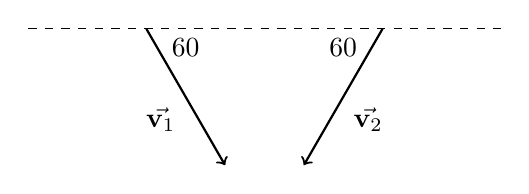
\begin{tikzpicture}
    \draw[dashed] (-3,0) -- (3,0);
    \draw[thick,->] (-1.5,0) -- ++(300:2) node[anchor=north east,pos=0.5] {$\vec{\mathbf{v}_1}$};
    \node[anchor=north west] at (-1.30,0) {\ang{60}};
    \draw[thick,->] (+1.5,0) -- ++(240:2) node[anchor=north west,pos=0.5] {$\vec{\mathbf{v}_2}$};
    \node[anchor=north east] at (+1.30,0) {\ang{60}};
\end{tikzpicture}
}

\element{serway-mc}{
\begin{question}{serway-ch09-q79}
    Two birds of prey hurtling after the same mouse collide in mid-air and grab each other with their talons.
    \begin{center}
        \serwayChNineQSeventyNine
    \end{center}
    If each \SI{250}{\gram} bird is flying at \SI{30}{\meter\per\second} at a \ang{60} angle to the ground,
        what is their total momentum immediately after the collision?
    \begin{multicols}{3}
    \begin{choices}
        \wrongchoice{zero}
        \wrongchoice{\SI{6.5}{\kilo\gram\meter\per\second}}
        \wrongchoice{\SI{7.5}{\kilo\gram\meter\per\second}}
      \correctchoice{\SI{13}{\kilo\gram\meter\per\second}}
        \wrongchoice{\SI{15}{\kilo\gram\meter\per\second}}
    \end{choices}
    \end{multicols}
\end{question}
}

\element{serway-mc}{
\begin{question}{serway-ch09-q80}
    Two birds of prey hurtling after the same mouse collide in mid-air and grab each other with their talons.
    \begin{center}
        \serwayChNineQSeventyNine
    \end{center}
    If each \SI{250}{\gram} bird is flying at \SI{30}{\meter\per\second} at a \ang{60} angle to the ground,
        what is the magnitude of their velocity immediately after the collision?
    \begin{multicols}{3}
    \begin{choices}
        \wrongchoice{zero}
        \wrongchoice{\SI{13}{\meter\per\second}}
        \wrongchoice{\SI{15}{\meter\per\second}}
      \correctchoice{\SI{26}{\meter\per\second}}
        \wrongchoice{\SI{30}{\meter\per\second}}
    \end{choices}
    \end{multicols}
\end{question}
}

\element{serway-mc}{
\begin{question}{serway-ch09-q81}
    Two birds of prey hurtling after the same mouse collide in mid-air and grab each other with their talons.
    \begin{center}
        \serwayChNineQSeventyNine
    \end{center}
    If each \SI{250}{\gram} bird is flying at \SI{30}{\meter\per\second} at a \ang{60} angle to the ground,
        what is the horizontal componenet of their momentum immediately after the collision?
    \begin{multicols}{3}
    \begin{choices}
      \correctchoice{zero}
        \wrongchoice{\SI{6.1}{\meter\per\second}}
        \wrongchoice{\SI{7.5}{\meter\per\second}}
        \wrongchoice{\SI{13}{\meter\per\second}}
        \wrongchoice{\SI{15}{\meter\per\second}}
    \end{choices}
    \end{multicols}
\end{question}
}

\element{serway-mc}{
\begin{question}{serway-ch09-q82}
    A \SI{500}{\gram} firework explodes into two pieces of equal mass at an instant when it is traveling straight up at \SI{10}{\meter\per\second}.
    If one half shoots off horizontally to the left at \SI{20}{\meter\per\second},
        what is the velocity of the other half immediately after the explosion?
    (The $x$-axis is directed right; the $y$-axis up.)
    \begin{multicols}{2}
    \begin{choices}
        \wrongchoice{$\left(-20\hat{\imath}-20\hat{\jmath}\right)\,\si{\meter\per\second}$}
        \wrongchoice{$\left(-20\hat{\imath}+20\hat{\jmath}\right)\,\si{\meter\per\second}$}
        \wrongchoice{$\left(+20\hat{\imath}-20\hat{\jmath}\right)\,\si{\meter\per\second}$}
      \correctchoice{$\left(+20\hat{\imath}+20\hat{\jmath}\right)\,\si{\meter\per\second}$}
        \wrongchoice{$\left(-20\hat{\imath}+20\hat{k}\right)\,\si{\meter\per\second}$}
    \end{choices}
    \end{multicols}
\end{question}
}


\endinput


